% Тут используется класс, установленный на сервере Papeeria. На случай, если
% текст понадобится редактировать где-то в другом месте, рядом лежит файл matmex-diploma-custom.cls
% который в момент своего создания был идентичен классу, установленному на сервере.
% Для того, чтобы им воспользоваться, замените matmex-diploma на matmex-diploma-custom
% Если вы работаете исключительно в Papeeria то мы настоятельно рекомендуем пользоваться
% классом matmex-diploma, поскольку он будет автоматически обновляться по мере внесения корректив
%

% По умолчанию используется шрифт 14 размера. Если нужен 12-й шрифт, уберите опцию [14pt]
\documentclass[14pt]{matmex-diploma}
%\documentclass[14pt]{matmex-diploma-custom}

\begin{document}
% Год, город, название университета и факультета предопределены,
% но можно и поменять.
% Если англоязычная титульная страница не нужна, то ее можно просто удалить.
\filltitle{ru}{
    chair              = {Программная инженерия},
    title              = {Анализ решений задачи о подсчете количества треугольников в графе, основанных на линейной алгебре},
    % Здесь указывается тип работы. Возможные значения:
    %   coursework - Курсовая работа
    %   diploma - Диплом специалиста
    %   master - Диплом магистра
    %   bachelor - Диплом бакалавра
    type               = {coursework},
    position           = {студента},
    group              = 271,
    author             = {Погожельская Влада},
    supervisorPosition = {к.\,ф.-м.\,н., доцент},
    supervisor         = {Григорьев С.\,В.},
%   university         = {Санкт-Петербургский Государственный Университет},
%   faculty            = {Математико-механический факультет},
%   city               = {Санкт-Петербург},
%   year               = {2020}
}
\maketitle
\tableofcontents
% У введения нет номера главы
\section*{Введение}
Анализ больших данных является важной областью современных научных исследований. Многие задачи из этой области естественным образом выражаются в терминах графов. Данные, представленные в виде графа, могут отражать отношения между людьми в социальных сетях, биологические или генетические взаимодействия или, например, отображать сеть цитирования в Интернете. В связи с широкой областью их применения, понимание базовой структуры графа становится все более важной задачей при разработке эффективных алгоритмов анализа больших данных.

Важным направлением изучения структуры графов является поиск в нём некоторых шаблонных подграфов, иначе говоря, subgraph matching. Одним из наиболее часто используемых является треугольник.

Подсчет количества треугольников в графе --- это проблема нахождения количества уникальных троек вершин $u, v, w$ в неориентированном графе, таких что $(u, v), (u, w), (v, w) \in E$, где $E$ --- множество ребер графа. Данная задача может быть применена в анализе социальных сетей, где используется для обнаружения сообществ и степени сплоченности между ними. Также, на этой мере основаны такие важные характеристики в анализе сетей, как коэффициент кластеризации и коэффициент транзитивности.

Растущая потребность использования данного алгоритма как структурного элемента в прикладных задачах актуализирует исследования по его ускорению и увеличению масштабируемости при запуске на больших параллельных системах.

Однако, по мере роста количества вершин и ребер в графе, возникает вопрос об эффективной параллельной обработке данных. Благодаря высокой степени параллелизма и высокой пропускной способности доступа к памяти, графические процессоры все чаще начали применять в неграфических вычислениях. Впоследствии, графические процессоры были адаптированы для ускорения обработки графов больших размеров и для них был разработан ряд алгоритмов. Но, несмотря на это, высокопроизводительные графовые алгоритмы всё еще требует больших трудозатрат со стороны программиста по реализации как на GPU, так и на CPU, так как зачастую для их эффективного использования необходимо знать аппаратные особенности. Для решения данной проблемы было разработано несколько библиотек, предоставляющих высокоуровневый интерфейс и помогающих лаконично выражать графовые алгоритмы. Многие из них базируются на представлении графовых алгоритмов в терминах линейной алгебры. Задача подсчета количества треугольников не стала исключением и для ее решения было реализовано несколько матричных алгоритмов с помощью различных библиотек. Так как данные разработки в первую очередь были направлены на обработку графов, которые возникают в реальной жизни, то важной частью является анализ применимости данных результатов на практике.

В данной работе планируется провести сравнение и анализ существующих на данный момент решений задачи подсчета количества треугольников, основанных на линейной алгебре.

\section{Постановка задачи}
Целью данной работы является сравнительный анализ существующих на данный момент решений задачи подсчета количества треугольников, основанных на линейной алгебре.
Для достижения цели были выделены перечисленные ниже задачи.
\begin{itemize}
    \item Выполнить обзор существующих решений задачи о подсчете количества треугольников, основанных на линейной алгебре, и использованных для этого инструментов. Целью обзора является: выбрать алгоритмы, которые необходимо реализовать для полноты планируемого сравнения и выбрать подходящую библиотеку для реализации.
    \item Выполнить реализацию выбранного алгоритма подсчета количества треугольников в графе с помощью выбранной библиотеки.
    \item Провести экспериментальное исследование реализованного алгоритма и уже существующих в данной библиотеке.
\end{itemize}

\section {Обзор существующих решений и библиотек}
В последние годы вследствие быстрого роста размеров графов, которые необходимо анализировать, были проведены серьезные исследования в области повышения производительности алгоритмов подсчета количества треугольников в графе. В этом разделе будут кратко описаны основные подходы к решению этой задачи в контексте ее реализации в терминах линейной алгебры. Также будут рассмотрены использованные при этом библиотеки и их особенности.

Для дальнейшего описания алгоритмов обозначим за $A$ --- булеву симметричную матрицу смежности входного графа, $L$ --- верхнетреугольную матрицу от $A$, а $U$ --- нижнетреугольную ($A = L + U$); (*) --- оператор стандартного умножения матриц, (.*) --- оператор поэлементного умножения матриц, (') --- транспонирование матрицы.

\begin{itemize}
\item \textbf{Базовая версия матричного алгоритма}

Количество треугольников в графе выражается формулой:\\ $\frac{1}{6}trace(A^{3})$, где $trace$ --- след матрицы, выражающийся формулой $trace(A) = \sum_{i}a_{ii}$.

\item \textbf {Burkhardt algorithm}

 Алгоритм отличается от базового тем, что одна из операций умножения матриц заменена менее "тяжеловесной" операцией поэлементного умножения. Итоговое количество треугольников: \\  $\frac{1}{6} \sum\limits_j (\sum\limits_i ((A^{2}) .* A))$.
 
\item \textbf{Cohen algorithm}

Данный алгоритм подсчета количества треугольников основан на алгоритме MapReduce, автором которого является J.Cohen ~\cite{Cohen}. Идея реализованного алгоритма заключается в следующем:
\begin{itemize}
    \item Разбить матрицу смежности $A$ на верхнетреугольную матрицу $L$ и нижнетреугольную матрицу $U$.
    \item Посчитать матрицу $B = LU$.
    \item Наконец, $C = A \circ B$ (поэлементное умножение).
       
      Тогда, итоговое количество треугольников ---  $\frac{1}{2}\sum\limits_i\sum\limits_j C_{ij}$.
      
      Данный алгоритм использует менее тяжеловесные операции умножения матриц, однако, каждый треугольник в итоге будет посчитан дважды.
\end{itemize}

\item \textbf{Sandia algorithm}

Данный алгоритм является последним по времени разработки и является наиболее производительным. Данный алгоритм базируется на следующей формуле: $sum (sum ((U * U) .* U))$, при этом каждый треугольник будет посчитан единожды.
\item  \textbf{SandiaDot algorithm}

Метод SandiaDot аналогичен Sandia, но опирается на тот факт, что $L = U'$, так как матрица $A$ симметричная, и не транспонирует матрицу $U$ явно. Тогда итоговая формула, использующаяся в алгоритме: $sum (sum ((L * U') .* L))$
\end{itemize}

Из обзора подходов к решению задачи с помощью линейной алгебры видно, что базовый алгоритм имеет большие просторы для оптимизаций и ускорения засчёт уменьшения количества умножений и повышения их эффективности (использование верхне- или нижнетреугольной матрицы вместо полной). Однако, также важным фактором целесообразности использования того или иного алгоритма в реальных условиях является не только его эффективность, но и воспроизводимость --- то, насколько кратко и лаконично позволяют описать его современные инструменты. С этой целью были рассмотрены следующие библиотеки.

\begin{itemize}
    \item \textbf{GraphBLAS Template Library (GBTL)}

GBTL ~\cite{Zhang2016GBTLCUDAGA} --- реализация открытого стандарта GraphBLAS для языка C++. GraphBLAS --- это новая парадигма для обработки графов, которая облегчает разработку графовых алгоритмов, выражая их в терминах линейной алгебры. Важно отметить, что графовый алгоритм, написанный согласно этому стандарту, может выполняться в самых разных средах программирования, от встроенных сред до компьютеров с распределенной памятью. В данной библиотеке содержится реализация алгоритма Cohen, однако, в ней не поддерживается вычисления на GPU.

\item \textbf{GraphBLAST}

GraphBLAST~\cite{gr} --- высокопроизводительный фреймворк с открытым исходным кодом, помогающий реализовывать графовые алгоритмы в терминах линейной алгебры. Библиотека GraphBLAST представляет особенный интерес для реализации графовых алгоритмов, так как совмещает в себе Gunrock \cite{gunrockmodel} в качестве backend’а и компактный и простой в использовании пользовательский интерфейс стандарта GraphBLAS. На данный момент алгоритм подсчета количества треугольников в графе не поддерживается библиотекой. Однако, разработчиками утверждается, что основной код реализации занимает 6 строк и по крайней мере, не уступает по производительности реализациям использующих другие графовые фреймфорки ~\cite{gbarticle}.

     
    \item \textbf{SuiteSparse:GraphBLAS} 

SuiteSparse:GraphBLAS --- фреймворк так же полностью соответствует стандарту GraphBLAS, при этом дополнен поддержкой операций с разреженными матрицами над расширенной алгеброй полуколец. Применительно к разреженным матрицам смежности эти алгебраические операции эквивалентны вычислениям на графах. Стоит отметить, что GraphBLAS предоставляет мощную и выразительную основу для создания графовых алгоритмов, основанных на изящной математике разреженных матричных операций в полукольце.

В примерах библиотеки представлены все выше описанные алгоритмы решения задачи подсчета количества треугольников, кроме базового. Все они оптимизированы для быстрого умножения разреженных матриц с помощью методов, предоставляемых библиотекой. На сегодняшний день поддерживаемые ей реализации алгоритмов подсчета треугольников SuiteSparse показывают наиболее высокие результаты по сравнению с другими графовыми фреймворками \cite{suitesparse}.

\end{itemize}

В результате анализа существующих решений были выявлены особенности реализации алгоритмов подсчета треугольников в зависимости от используемых технологий. Графовые алгоритмы удобно представлять в терминах линейной алгебры по крайней мере по двум причинам. Во-первых, многие алгоритмы, в том числе и подсчет количества треугольников, кратко и лаконично выражаются через матричное представление. Во-вторых, как было показано выше на примере SuiteSparse, для них реализованы эффективные алгоритмы. Тем не менее, вопрос о практической применимости базового алгоритма остается открытым, так как ни в одной из представленных библиотек не был реализован базовый алгоритм для решения задачи подсчета количества треугольников в графе, хотя сравнение оптимизированных алгоритмов с ним является показательным с точки зрения эффективности примененных оптимизаций. По этим причинам этот алгоритм был выбран для дальнейшей реализации.

\section{Реализация}

Как было показано в предыдущем разделе, решение проблемы подсчета количества треугольников поддерживается несколькими библиотеками, позволяющими выразить алгоритм через матричное представление. В ходе изучения библиотек изначально было принято решение реализовывать базовый алгоритм с помощью библиотеки GraphBLAST. Однако, в процессе сборки и тестирования ее существующих компонент и уже написанных в качестве демо алгоритмов был обнаружен ряд проблем, не позволяющих реализовать стабильно работающую версию алгоритма. О найденных ошибках было сообщено разработчикам в виде issues в репозитории библиотеки. Так как быстрого решения проблем не ожидалось, то в качестве альтернативной библиотеки для реализации алгоритма была выбрана наиболее стабильная и производительная на сегодняшний день библиотека, соответствующая стандарту GraphBLAS --- SuiteSparse. Эта библиотека "заточена" под работу над разреженными матрицами, которые наиболее часто возникают в реальных графах. Также, для дальнейшего проведения экспериментального сравнения необходимо обеспечить соответствующую архитектуру решения. 


\subsection{Базовый алгоритм}

Проблема подсчета количества треугольников имеет множество путей решения. В том числе, было разработано несколько алгоритмов, основанных на матричных операциях. В библиотеке SuiteSparse поддерживается 4 метода решения задачи, отличающихся по использованию памяти и времени работы.

В рамках данной работы был реализован еще не представленный в библиотеке метод, который, тем не менее, является наиболее известным подходом к решению задачи в терминах линейной алгебры. 

Дан неориентированный граф $G = (V, E)$ без петель и кратных ребер, где $V$ --- множество вершин графа, $|V| = N$, $E$ --- множество ребер. Пусть $A$ --- матрица смежности, размером $N \times N$ со значениями 0 и 1, причем она симметрична и имеет все нули на диагонали. Если вычислить $A^n$, то $A^n[i][j]$ будет представлять собой количество различных путей в графе из $i$ в $j$ длины n. Соответственно, для того, чтобы найти пути длины 3, необходимо вычислить $A^3$. При этом, значение $A^3[i][i]$ отображает количество путей, начинающийся и заканчивающийся в вершине $i$, что и есть количество треугольников, проходящих через вершину $i$. Так как число треугольников считается для каждой вершины и каждый треугольник будет посчитан трижды, то общее количество необходимо разделить на 3, так же, так как граф неориентированный, делим еще на 2. Итого, число треугольников в графе можно выразить в виде формулы: $\frac{1}{6} trace(A^{3})$. Данный алгоритм является "наивным" и его асимптотическая сложность составляет $\mathcal{O}(N^3)$, а объем занимаемой памяти --- размер матрицы $A$.
 
\subsection{Особенности реализации с помощью \\ SuiteSparse:GraphBLAS}
Особенность реализации данного алгоритма на SuiteSparse состоит в том, что функция перемножения двух разреженных матриц $GrB\_mxm$ использует полукольцо. Поэтому сначала необходимо сконструировать коммутативный и ассоциативный моноид по сложению и далее сконструировать из него полукольцо по умножению.

    Моноиды в SuiteSparse: скалярное сложение в стандартном умножении матриц заменяется моноидом. Моноид ($GrB\_Monoid$) является ассоциативным и коммутативным бинарным
оператором $z = f(x; y)$, где х, у и z одинакового типа и оператор имеет
нейтральный элемент $e$ такой, что $f(x; e) = f(e; x) = x$.

Полукольца в SuiteSparse: Полукольцо ($GrB\_Semiring$) состоит из
моноида и оператора «умножения». Вместе эти операции
определяют операцию матричного умножения  $C = AB$, где
моноид используется как аддитивный оператор и полукольцо используется как оператор «умножения» вместо стандартного скалярного умножения. SuiteSparse дает возможность определять свои собственные моноиды и полукольца.

В библиотеку встроены несколько алгоритмов умножения матриц, в том числе те, у которых асимптотическое время работы меньше, чем $\mathcal{O}(N^3)$, из чего следует улучшение асимптотики работы алгоритма подсчета количества треугольников. В данной реализации был использован оптимизированный метод умножения матриц --- Gustavson's method ~\cite{Gustavson}.

\subsection{Архитектура решения}
Для проведения экспериментального исследования реализованного алгоритма и уже существующих была разработана система, позволяющая автоматизировать процесс сборки, запуска и замеров времени работы алгоритмов. На рисунке 1 представлена архитектура реализованного решения.

Данная система состоит из:
\begin{itemize}
\item скрипта test.py, написанного на Python;
\item исходных файлов main.c, mytricount.c, timer.c;
\item библиотеки SuiteSparse: GraphBLAS.
\end{itemize}

\begin{figure}[h!]
	\centering
	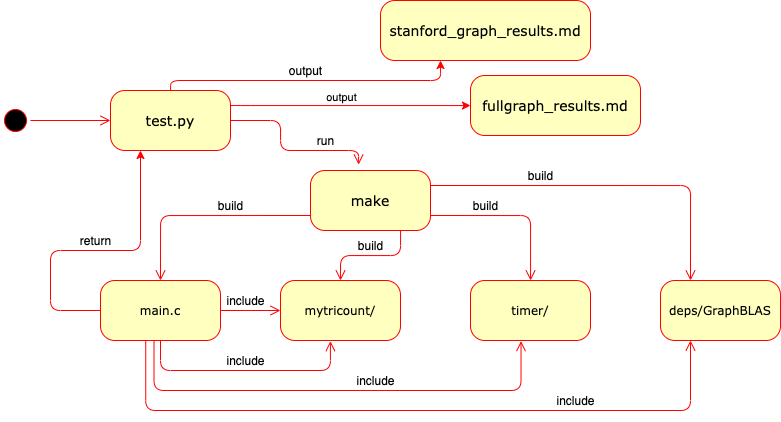
\includegraphics[width=\columnwidth]{pics/arch1.png}
	\caption{Архитектура решения}
	\label{fig:Архитектура}
\end{figure}
Для старта алгоритма необходимо запустить скрипт test.py,  внутри которого последовательно вызывается:
    \begin{enumerate}
        \item Сборка исходных файлов с помощью make.
        \subitem В файле main.c выполняется загрузка графа и запуск реализованного алгоритма и уже существующих в библиотеке алгоритмов подсчета количества треугольников на реальных и полных графах вместе с замерами времени.
        \subitem В папке mytricount лежит файл с исходным кодом алгоритмов и заголовочный файл к нему.
        \subitem В папке timer лежит файл с исходным кодом таймера для замера производительности и заголовочный файл у нему.
        \subitem В deps находится исходный код самой библиотеки SuiteSparse: GraphBLAS. 
        \item Загрузка графов, представляющих собой реальные данные, в папку input \footnote{Графы доступны по ссылке: ~\cite{data} }.
        \item Генерация полных графов и сохранение их в ту же папку.
        \item Запуск собранного с помощью make исполняемого файла.
        \item Запись результатов замеров в две итоговые таблицы отдельно для реальных и полных графов.
    \end{enumerate}
    

\section{Cравнительный анализ}
В данном разделе приведен сравнительный анализ результатов работы алгоритма на различных графах. Для его проведения использовалось два типа графов: сгенерированные полные графы и реальные графы, которые возникают на практике и являются довольно разреженными. В таблице данные представлены в секундах.
 
В таблице 1 приведены результаты замеров алгоритмов на полных графах. В ней можно увидеть, что наивный алгоритм показывает сравнимые с оптимизированными алгоритмами результаты времени работы даже с ростом количества вершин и разница времени его работы с остальными алгоритмами сохраняется на том же уровне по мере роста количества вершин в графе. Однако, полные графы в реальной жизни возникают достаточно редко, поэтому полученные результаты на синтетических графах ничего не говорят о практической применимости. Также, поддерживаемые библиотекой алгоритмы являются оптимизированными для работы с большими разреженными матрицами, что означает, что плотный граф с небольшим количеством вершин является для них худшим случаем и их время работы может приближаться к базовому алгоритму.

В таблице 2 приведены результаты замеров работы алгоритмов на реальных графах. Определенно, запуск "наивного" алгоритма на реальных графах явно показал, что он сильно проигрывает другим алгоритмам и количество работы, выполняемое им, не является оптимальным. Методы Burkhardt и Cohen намного более эффективны по сравнению с "наивным" методом, но при этом занимают пространство в памяти того же размера, то есть размера матрицы $A$. С другой стороны, они работают медленнее, чем метод Sandia, который занимает немного меньше памяти, чем Burkhardt и Cohen, и, безусловно, является самым быстрым среди всех представленных алгоритмов. При этом, модернизация последнего алгоритма почти ни на одном графе не дала выигрыша по времени.

В результате сравнительного анализа можно смело делать выводы о том, что проведенные оптимизации базового алгоритма дали существенный прирост в производительности на графах, отражающих реальные данные и задачи, а базовый алгоритм есть смысл применять только на полных или очень плотных графах. Из всех рассмотренных алгоритмов наиболее эффективным во всей сценариях показал себя алгоритм Sandia, в пользу которого следует делать выбор на практике при необходимости решить задачу подсчета количества треугольников лаконичным и при этом эффективным способом.

 \clearpage
  \begin{table}[h]
\caption{Результаты замеров на полных графах}
\begin{center}
\begin{tabular}[c]{|l|l|l|l|l|l|}
\hline
\textbf{N} &
  \textbf{\begin{tabular}[c]{@{}l@{}}Naive\end{tabular}} &
  \textbf{\begin{tabular}[c]{@{}l@{}}Burkhardt\end{tabular}} &
  \textbf{\begin{tabular}[c]{@{}l@{}}Cohen\end{tabular}} &
  \textbf{\begin{tabular}[c]{@{}l@{}}Sandia\end{tabular}} &
  \textbf{\begin{tabular}[c]{@{}l@{}}SandiaDot\end{tabular}} \\ \hline
10   &  < 0.001  & < 0.001  & < 0.001 & < 0.001 & < 0.001   \\ \hline
50   & 0.002  & < 0.001 & < 0.001 & < 0.001 & < 0.001   \\ \hline
100  & 0.002  & 0.002  & < 0.001 & < 0.001 & < 0.001  \\ \hline
200  & 0.014  & 0.017  & 0.002 & 0.001 & 0.003  \\ \hline
300  & 0.048  & 0.021  & 0.007 & 0.004 & 0.011   \\ \hline
400  & 0.112  & 0.048  & 0.017 & 0.010 & 0.025   \\ \hline
500  & 0.217  & 0.107  & 0.033 & 0.017 & 0.048   \\ \hline
600  & 0.392  & 0.167  & 0.064 & 0.029 & 0.082   \\ \hline
700  & 0.611  & 0.261  & 0.089 & 0.045 & 0.134   \\ \hline
800  & 0.924  & 0.402  & 0.144 & 0.067 & 0.201   \\ \hline
900  & 1.356  & 0.589  & 0.203 & 0.094 & 0.284   \\ \hline
1000 & 1.915  & 0.820  & 0.251 & 0.129 & 0.382   \\ \hline
\end{tabular}
\end{center}
\end{table}

\begin{table}[h!]
\caption{Результаты замеров на реальных графах}
\begin{center}
\resizebox{\textwidth}{!}{%
\begin{tabular}{|l|l|l|l|l|l|l|l|l|}
\hline
\textbf{Name} &
  \textbf{\begin{tabular}[c]{@{}l@{}}nodes\\ $\times 10^{6}$\end{tabular}} &
  \textbf{\begin{tabular}[c]{@{}l@{}}edges\\ $\times 10^{6}$\end{tabular}} &
  \textbf{\begin{tabular}[c]{@{}l@{}}Naive\end{tabular}} &
  \textbf{\begin{tabular}[c]{@{}l@{}}Burkhardt\end{tabular}} &
  \textbf{\begin{tabular}[c]{@{}l@{}}Cohen\end{tabular}} &
  \textbf{\begin{tabular}[c]{@{}l@{}}Sandia\end{tabular}} &
  \textbf{\begin{tabular}[c]{@{}l@{}}SandiaDot\end{tabular}} \\ \hline
loc-brightkite\_edges & 0.06 & 0.21  & 5.880  & 0.050 & 0.030 & 0.018 & 0.016 \\ \hline
amazon0302 & 0.40 & 2.35 & 2.220 & 0.111 & 0.063 & 0.034 & 0.035 \\ \hline
roadNet-PA & 1.09 & 1.54 & 0.351  & 0.045 & 0.075 & 0.053 & 0.032 \\ \hline
amazon0505 & 0.41 & 2.44 & 28.143 & 0.480 & 0.270 & 0.095 & 0.111 \\ \hline
soc-Epinions1 & 0.08 & 0.41 & 33.430 & 0.146 & 0.060 & 0.035 & 0.052 \\ \hline
email-EuAll & 0.27 & 0.36 & NaN & 0.333 & 0.111 & 0.019 & 0.040 \\ \hline
loc-gowalla\_edges & 0.20 & 0.95 & NaN & 0.484 & 0.303 & 0.116 & 0.097 \\ \hline
soc-Slashdot0902 & 0.08 & 0.50 & 50.605 & 0.168 & 0.075 & 0.039 & 0.057 \\ \hline
soc-Slashdot0811 & 0.08 & 0.47 & 47.451 & 0.152 & 0.068 & 0.035 & 0.053 \\ \hline
\end{tabular}%
}
\end{center}
\end{table}
 \clearpage \section{Заключение}
В рамках данной работы были выполнены следующие задачи:
\begin{itemize}
    \item Выполнен обзор существующих решений задачи о подсчете количества треугольников, основанных на линейной алгебре, и использованных для этого инструментов. Выбран алгоритм и библиотека.
    \item Выполнена реализация выбранного алгоритма подсчета количества треугольников в графе с помощью библиотеки GraphBLAS: SuiteSparse.
    \item Проведено экспериментальное исследование реализованного алгоритма и уже существующих в данной библиотеке.
\end{itemize}

В качестве дальнейшего исследования возможна реализация описанных алгоритмов с помощью библиотеки GraphBLAST и экспериментальное сравнение их производительности с полученными результами в данной работе.
\setmonofont[Mapping=tex-text]{CMU Typewriter Text}
\bibliographystyle{ugost2008ls}
\bibliography{coursework.bib}
\end{document}